\section{Werkzeuge und Technologien}
\subsection{Unterschied zwischen ReactJS und React Native}
ReactJS und React Native haben zwar sehr viele Gemeinsamkeiten, jedoch auch einige Unterschiede.
Während ReactJS eine JavaScript-Bibliothek ist, ist React Native ein vollständiges Framework. Dies bedeutet, dass bereits beim Setup alles mitgeliefert wird, was für die
Entwicklung notwendig ist. Weitere Unterschiede sind der DOM und das Styling. Während die Komponenten in ReactJS als HTML gerendert werden, werden bei React Native - wie der Name schon andeutet - native UI-Elemente verwendet.
Beide Technologien verwenden hierfür \textit{JSX}.
Die Erweiterung von JavaScript ermöglicht eine XML-Beschreibung von Komponenten direkt im JavaScript-Code.

Der größte Unterschied ist die Plattform. ReactJS ist für Web-Applikationen in Browsern optimiert. Aus diesem Grund auch der HTML-Code. React Native hingegen speziell für native Applikationen auf Endgeräten.
Aus diesem Grund lässt sich bei React Native auch Nativer Code einbinden. Dies ist leider bei komplexeren Funktionen zwingend notwendig. Um mit den React-Konzepten eine Applikation außerhalb des
Browsers zu entwickeln ist demnach \textit{React Native} notwendig. \cite{ReactJSvsReactNative:online}

\subsection{Redux}
Redux ist ein Framework, das einen Container für die \textit{states} einer React-Anwendungen liefert. Durch die zentrale Verwaltung der States in einem \textit{App-State}
wird die React-Anwendung klarer strukturiert und leichter testbar.

\subsection{Zusammenspiel der Technologien}
In der Vorlesung wurde bereits das Prinzip von React Native erläutert. In \autoref{fig:ReduxReact} ist
der grobe Ablauf von React Native in Ergänzung mit Redux dargestellt. Es ergibt sich ein Kreislauf, der beispielsweise durch
eine Benutzeraktion getriggert wird.

Das UI besteht aus Komponenten. Bei einer Benutzeraktion
triggert das UI eine deklarativ beschriebene Aktion, welche vom Reducer aufgefangen wird.
Der Reducer kümmert sich unter anderem darum, dass der Store, welcher alle States beinhaltet, aktualisiert wird.
Sobald sich ein State ändert wird das UI neu gerendert und der Benutzer sieht das Ergebnis seiner Aktion.

\begin{figure}[h]
    \centering
    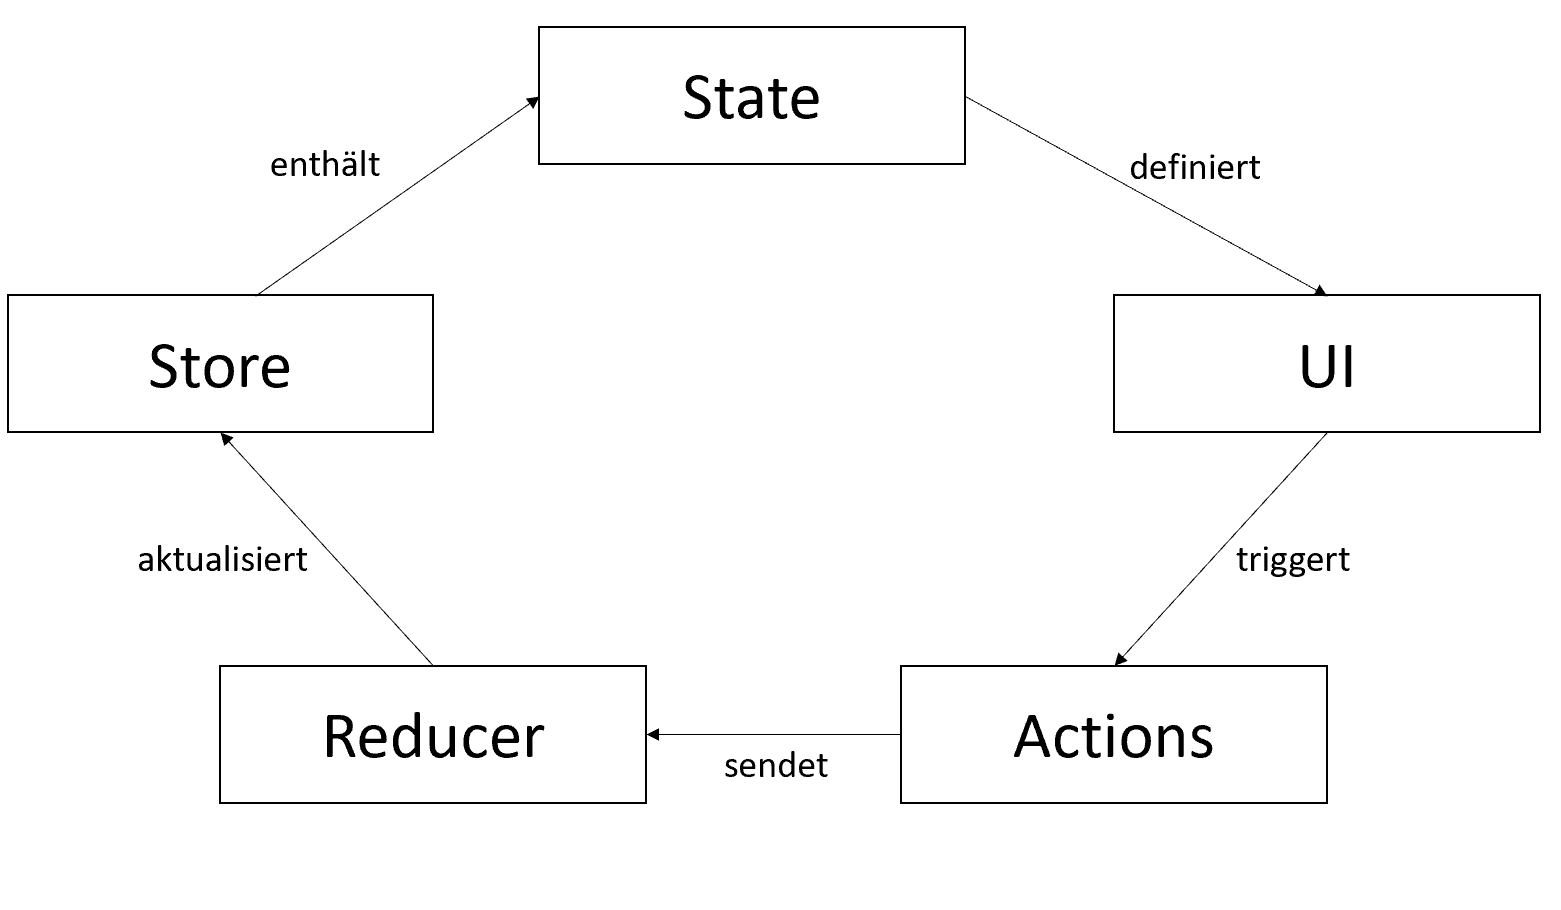
\includegraphics[width=10cm]{ReduxReactGrobAblauf.png}
    \caption{Ablauf: React und Redux}
    \label{fig:ReduxReact}
\end{figure}

Im Folgenden werden die einzelnen Bausteine, einschließlich der zusätzlichen Bibliothek \textit{Redux-Saga}, erläutert und
anschließend der detaillierte Ablauf beschrieben.

\paragraph{Store}
Der Store enthält den kompletten \textit{State-Tree}. Das bedeutet, dass jede Veränderung
eines \textit{States} im Store enthalten ist. Der Store ist damit der zentrale Knotenpunkt der Applikation.

\paragraph{Reducer}
Die Reducer sorgen für die Prozessierung der Aktionen. Sie enthalten die Logik, die
durch eine Aktion ausgeführt werden soll. Sobald eine Aktion getriggert wird, wird diese von einem
Reducer aufgefangen und eine Prozedur, die unter anderem den Store aktualisiert, wird ausgeführt.

\paragraph{Actions}
Die Aktionen sind rein deklarativ geschrieben. Das bedeutet, sie enthalten keine Ausführlogik,
sondern werden lediglich definiert. Dazu gehören der Typ und optionale Parameter.
Bei Verwendung von TypeScript wird zusätzlich ein Interface erstellt.

\paragraph{API}
Die API enthält Methoden für verschiedene Zugriffe nach Außen.
Hierzu zählen insbesondere Zugriffe auf Firebase.
Diese Methoden werden asynchron ausgeführt.

\paragraph{Sagas}
Da die API-Funktionen asynchron ablaufen sind diese schwierig durch Redux zu behandeln.
Die Bibliothek \textit{Redux-Saga} vereinfacht dies.
Hierfür ist für jede Aktion, welche asynchrone Aufrufe tätigt, eine Saga notwendig. Diese strukturiert die Aufrufe, beschreibt
die Reihenfolge und triggert \textit{Erfolgsaktionen}, welche anschließend im Reducer
verarbeitet werden.

\paragraph{Components}
Die Komponenten können größtenteils aus den zuvor beschriebenen Bibliotheken verwendet werden.
Um die Entwicklung zu vereinfachen können diese \textit{Basiskomponenten} zu komplexeren kombiniert werden.
Die Komponenten besitzen, durch React,
jeweils einen eigenen \textit{State}, welcher jedoch nur in Ausnahmen verwendet wird.
Das State-Management wird durch Redux in den Store verlagert.
Die Komponenten besitzen \textit{props} über die
Daten an die Komponente übergeben werden können.

\paragraph{Container}
Container verknüpfen den Redux-State mit dem \textit{props} der Komponenten. Für die Verknüpfung
kann der Container zwei Methoden enthalten:
\begin{itemize}
    \item \textit{MapStateToProps}: Diese Methode ist fast immer notwendig, da hier Teile des States mit den \textit{props} übergeben werden.
    \item \textit{MapDispatchToProps}: Diese Methode ist nur dann notwendig, wenn die Komponente Aktionen auslösen kann. Beispielsweise bei einem Input-Field.
    Die Methode triggert eine Aktion, die anschließend vom Reducer verarbeitet werden kann.
\end{itemize}

\paragraph{Screens}
Die Screens gruppieren die Container und stellen diese auf einer Seite dar.
Zwischen den Screens läuft die Navigation der Applikation ab.

\newpage
\paragraph{Ablauf von Redux-Saga}
\autoref{fig:ReduxSaga} stellt den Ablauf von Redux-Saga dar. Wird für eine Aktion beispielsweise ein Zugriff auf die Datenbank
benötigt, so leitet der Reducer diese an die Redux-Saga weiter. Die Saga ruft die Methode der API auf und wartet auf
die Antwort der Datenbank. Kommt die Antwort bei der Saga an, können weitere Aktionen ausgeführt und z.B. eine
\textit{Erfolgsmeldung} abgefeuert werden.

\begin{figure}[h]
    \centering
    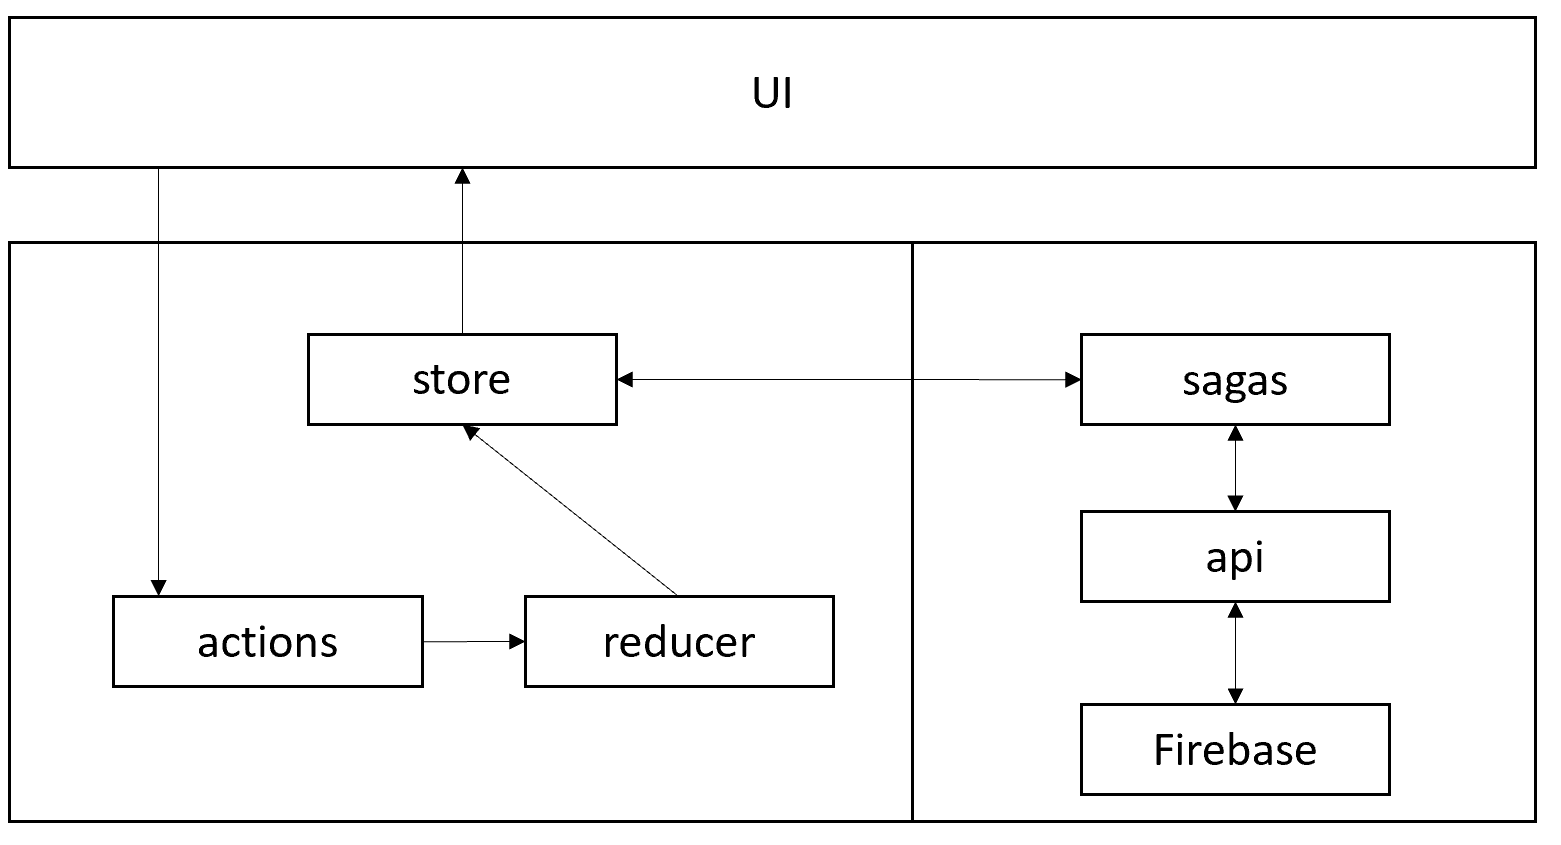
\includegraphics[width=\textwidth]{ReactReduxSaga.PNG}
    \caption{Ablauf: Redux-Saga}
    \label{fig:ReduxSaga}
\end{figure}

\subsection{TypeScript}
TypeScript bietet die Möglichkeit typisierten JavaScript-Code zu schreiben.
Durch die Typisierung wird die Entwicklung strukturierter und Objekte werden
klar definiert.

Neben der einfachen Typisierung bietet TypeScript weitere Möglichkeiten, die aus
objektorientierten Programmiersprachen, wie Java, bekannt sind.
Dies sind beispielsweise Interfaces und Klassen.

Die Verwendung von TypeScript bietet sich bei der Entwicklung von React Native-Apps an,
da das Framework die Typisierungen sehr gut unterstützt und auch die Unterstützung der React Native-Community sehr groß ist. \cite{TypescriptReasons:online}

\subsection{Verwendete Bibliotheken}
Im folgenden Abschnitt werden die in der Applikation verwendeten Bibliotheken kurz vorgestellt.

\paragraph{react}
Da \textit{React Native} auf React basiert, muss die React Bibliothek
in dem Projekt verfügbar sein. Das Konzept und der Ablauf wurden zuvor beschrieben. \cite{React:online}

\paragraph{react-native}
\textit{React Native} ist der Renderer (bzw. die Bridge), um aus dem JS-Code
die für die plattformspezifische Darstellung benötigten Komponenten zu erstellen.
\cite{ReactNative:online}

\paragraph{react-native-firebase}
Diese Bibliothek sorgt für eine einfach Anbindung der App zu Firebase. Hierfür wird eine leichtgewichtige
Schicht auf die Firebase SDK erstellt. Durch dieses Paket kann nach Konfiguration beispielsweise sehr leicht mit  \texttt{firebase.forestore()...} auf die
Datenbank zugegriffen werden.
\cite{invertas78:online}

\paragraph{native-base}
\textit{NativeBase} bietet
Komponenten für React Native, die plattformspezifische Designs umsetzen. Diese Komponenten erleichtern das Erstellen von Oberflächen und werden für die meisten UI-Komponenten der App
verwendet. \cite{NativeBase:online}

\paragraph{react-native-material-dialog}
NativeBase liefert leider keinen Dialog im Material Design, deshalb wird die Komponente zusätzlich als Package
importiert. Dieses Package liefert einen Dialog, der neben Items für den Inhalt eine \texttt{onCancel} und
\texttt{onOk} bereitstellt. Dies macht die Handhabung des Dialogs sehr simple. Der \textit{react-native-material-dialog}
wird in der Applikation für alle Dialoge verwendet.
\cite{MaterialDialog:online}

\paragraph{react-navigation}
Die \textit{react-navigation} bietet eine einfach zu verwendende Navigation für React Native.
Diese Navigation wird in der Applikation für die Navigation über das Menü und für die Navigation
direkt in bestimmte Screens verwendet. \cite{ReactNavigation:online}

\paragraph{redux}
\textit{Redux} bietet einen Container für die Verwaltung der States der einzelnen Komponenten.
In einer React Native App besitzt jede Komponente einen eigenen State. Um die Verwaltung dieser
States zu vereinfachen, wird Redux verwendet. Das Konzept von Redux wurde bereits zuvor beschrieben.
\cite{Redux:online}

\paragraph{react-redux}
Dieses Package ist notwendig, um Redux in einer React Native App zu verwenden und so die Vorteile von
Redux zu nutzen. Es verknüpft also React Native und Redux.
\cite{ReactRedux:online}

\paragraph{redux-form}
Die Bibliothek \textit{redux-form} unterstützt beim Verwalten des Redux-States in Formularen.
Dem Entwickler werden durch diese Bibliothek sehr viele Schritte abgenommen. Für die Formulare
gibt es einen eigenen \textit{Formreducer}, dieser aktualisiert die zu einer Action gehörenden States.
Der neue Status wird anschließend an das Feld, dass die Aktion gefeuert hat zurück gereicht. Dieser
Ablauf ist in \autoref{fig:ReduxForm} dargestellt. \cite{ReduxForm:online}

\begin{figure}[h]
    \centering
    \includegraphics[width=10cm]{ReduxFormDiagram.png}
    \caption{Ablauf: Redux-Form}
    \label{fig:ReduxForm}
\end{figure}

\paragraph{redux-saga}
\textit{Redux-Saga} wird für asynchrone Aktionen verwendet. Diese finden in dieser
App vor allem beim Zugriff auf Firebase statt. \cite{ReduxSaga:online,}

\paragraph{moment}
\textit{Moment.js} ist eine JavaScript-Bibliothek, die das Arbeiten mit Zeitdaten vereinfacht. Die Bibliothek ermöglicht es,
ein Datum zu formatieren, validieren und zu manipulieren. Dies ist besonders hilfreich bei der Auswertung und Darstellung der
Zeiterfassung. Das Datum muss hierzu in ein \textit{Moment} umgewandelt werden. \autoref{lst:moment-example} zeigt in einem kleinen Beispiel,
wie die Bibliothek in der Applikation verwendet wird. \cite{MomentJS:online}
\lstinputlisting[
    caption=Beispiel für Moment.js,
    label=lst:moment-example,
    language=Typescript,
    float=ht
]{moment.ts}

\paragraph{moment-duration-format}
Dies ist ein Plugin zusätzlich zu \textit{moment.js}. Dieses Plugin ist notwendig, da die Dauer ein anderes Format besitzt als ein Datum.
\textit{moment.js} ermöglicht zwar die Formatierung eines Datums,
allerdings nicht die einer Zeitdauer.
Das Plugin erweitert diese Funktionalität.
Es ermöglicht beispielsweise die Umwandlung einer Anzahl Stunden in Minuten.
In der Applikation wird dieses Format zur Darstellung der Zeiterfassungsergebnisse verwendet. \cite{MomentDuration:online}